W tym rozdziale prezentowany jest prototyp systemu wspomagania decyzji grupowej
TDM Team Decision Maker. Jest to oparta na architekturze klient-serwer
aplikacja internetowa, która implementuje teoretyczny model przedstawiony w
poprzednim rozdziale. Ze względu na złożoność systemu oraz samego modelu
teoretycznego na potrzeby tej pracy powstał jedynie prototyp, który wykorzystuje
tylko część funkcjonalności opisanych wcześniej. Niemniej jednak, jest to
wystarczające, aby zrozumieć zasadę działania oraz ideę systemu wspomagania
decyzji grupowej w warunkach dynamicznych.

W pierwszej części będzie omówiony aspekt informatyczny systemu,
czyli wykorzystane technologie, architektura oraz przepływ pracy (ang. work
flow), a także konkretne osadzenie modułów modelu teoretycznego.
Dalej opisany zostanie przypadek użycia wraz z wynikami obliczeń
wykonywanych przez system. Zobrazowana zostanie dynamika procesu oraz mobilność
rozwiązania. Możliwość uczestnictwa w procesie podejmowania decyzji bez
obowiązku fizycznej obecności w jednym miejscu, a nawet bez konieczności
zdalnego spotkania o określonej godzinie to jedna z większych zalet systemu.

Jednak głównym celem tego rozdziału, zaraz po samej prezentacji systemu, jest
podkreślenie tego, jak model matematyczny współgra z rzeczywistą implementacją i
zastosowaniem w praktyce. 

\section{Architektura systemu TDM}
Prototyp aplikacji TDM wykonany jest w architekturze klient-serwer, gdzie serwer
oparty jest na technologii JavaEE i udostępnia poprzez sieć usługi
wykorzystywane przez aplikacje klienckie. Do komunikacji został wykorzystany
wzorzec REST (ang. Representational State Transfer) oparty na protokole HTTP.
Dzięki temu system jest otwarty na powstawanie nowych aplikacji klienckich
napisanych w różnych technologiach. Na potrzeby tej pracy, w ramach prototypu,
jako klient wzorcowy powstała aplikacja przeglądarkowa. Ogólny diagram
architektury znajduje się na rysunku.
\missingfigure{Diagram architektury systemu}

\subsection{Wykorzystane technologie}
Głównym kryterium doboru technologii była możliwie jak największa dostępność
aplikacji na wszystkie nowoczesne urządzenia stacjonarne oraz, co ważniejsze,
mobilne (telefony, tablety). Istotną rzeczą była również łatwość wdrożenia
oprogramowania. Stąd też zdecydowano się na język Java wraz z platformą JavaEE
po stronie serwera, co zapewnia łatwą skalowalność i przenoszalność, oraz
na stronę internetową po stronie klienta, ponieważ większość obecnie dostępnych
urządzeń posiada zainstalowaną wydajną przeglądarkę internetową.

Lista zastosowanych technologii:
\begin{itemize}
  
  \item klient www
  \begin{itemize}
    \item Google Web Toolkit 3.5
    \item GWT-Platform 1.0-RC-3
    \item CSS 3
    \item GWT-Bootstrap 2.2.1.0
    \item Bootstrap from Twitter 2.3.1
    \item PhoneGap 2.7.0
  \end{itemize}
  
  \item serwer
  \begin{itemize}
    \item Google AppEngine 1.8.0
    \item Spring Framework 3.2.2
    \item Spring Security 3.1.3
    \item Spring Social 1.1.0
    \item Java Data Objects 3.0
    \item DataNucleus 3.1.1
    \item Scala 2.10.1
  \end{itemize}
\end{itemize}

\subsection{Aplikacja kliencka}
Powstałe w ramach prototypu oprogramowanie klienckie to strona internetowa
stworzona w technice AJAX (ang. Asynchronous JavaScript and XML) oraz SPA (ang.
single-page application). Całość została napisana w Google Web Toolkit,
platformie programistycznej pozwalającej na pisanie w języku Java i kompilację
do JavaScript. 

Wykorzystane technologie oraz techniki pozwoliły doskonale przystosować
aplikację nie tylko do użytku na standardowych przeglądarkach internetowych,
ale, co ważniejsze, na urządzeniach mobilnych. Brak potrzeby przeładowywania
strony oraz niewielka ilość danych otrzymywanych od serwera wpasowuje się w
ograniczony dostęp do Internetu oraz możliwości przeglądarki na tego typu
systemach.

Poniżej opisane są podstawowe ekrany oraz interakcja z użytkownikiem.

\subsubsection{Autentykacja}
Po wejściu na stronę aplikacji w przeglądarce, jako pierwszy pojawi się ekran
autentykacji. W ramach prototypu zrezygnowano z zarządzania kontami i możliwości
rejestracji. Jedynym sposobem dostępu do TDM jest skorzystanie z posiadanego
konta Google albo konta z serwisu społecznościowego Facebook. Docelowo aplikacja
będzie integrować się z serwisami społecznościowymi w celu pobrania informacji
na temat eksperta (np. zainteresowania, ulubione miejsca) oraz listy znajomych,
których może zaprosić do pomocy w rozwiązaniu problemu lub podjęciu decyzji.
\begin{figure}[!htbp]
  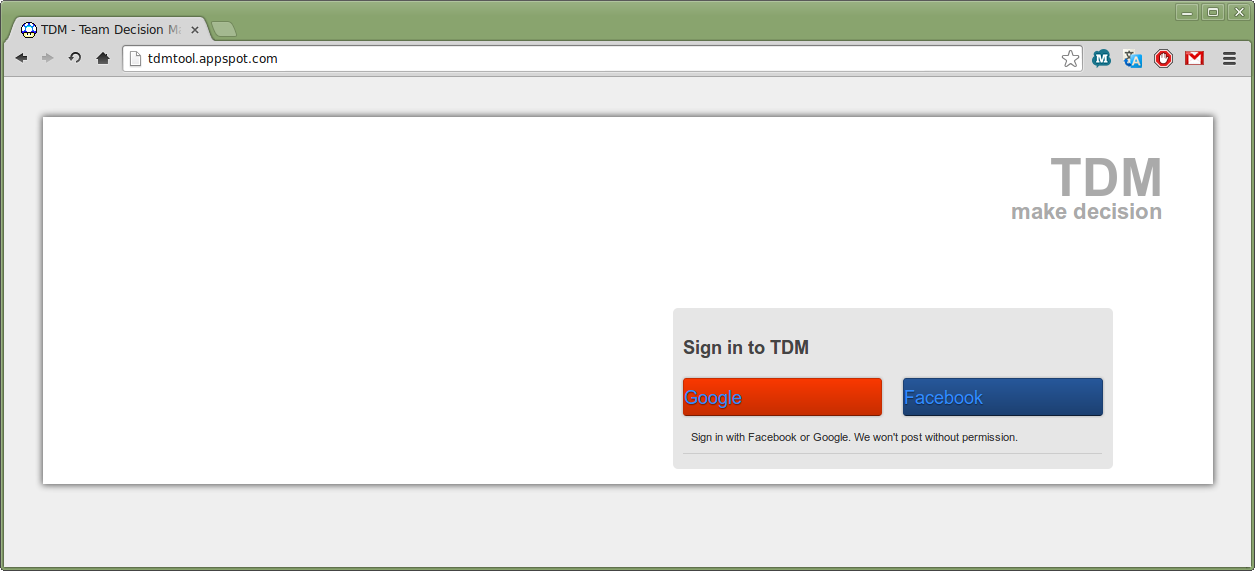
\includegraphics[width=\linewidth]
    {chapters/prototyp/tdm_authentication}
  \caption{Autentykacji do aplikacji TDM}
  \label{fig:authentication}
\end{figure}

\subsubsection{Lista problemów}
\begin{figure}[!htbp]
  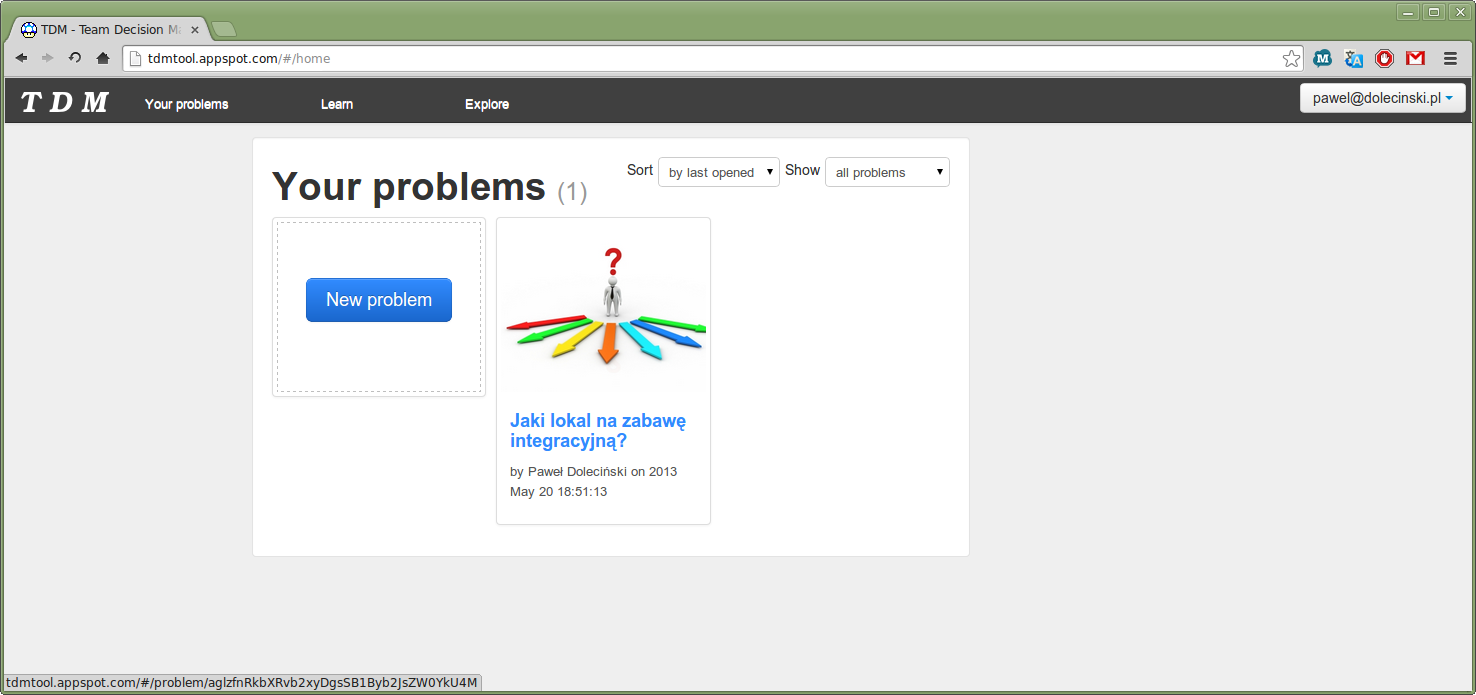
\includegraphics[width=\linewidth]
    {chapters/prototyp/tdm_problem_list}
  \caption{Lista aktualnych problemów decyzyjnych}
  \label{fig:problem_list}
\end{figure}

Po zalogowaniu użytkownik zobaczy ekran z dostępną listą problemów decyzyjnych
do rozwiązania. W tym miejscu widać elementy stworzone przez zalogowanego
eksperta oraz te, do których został zaproszony. Na tym ekranie można również
rozpocząć całkowicie nowy proces decyzyjny poprzez wybranie opcji ,,New
problem''. Wyświetlone zostanie okno dialogowe z prośbą o podanie nazwy problemu
oraz jego opcjonalnego opisu (rysunek \ref{fig:new_problem}). Jak widać,
aplikacja stara się jak najbardziej uprościć proces, a tym samym go
przyspieszyć. Stąd wszystkie techniczne parametru opisu problemu przyjmują
optymalne dla większości przypadków wartości domyślne z możliwością późniejszej
modyfikacji.

\begin{figure}[!htbp]
  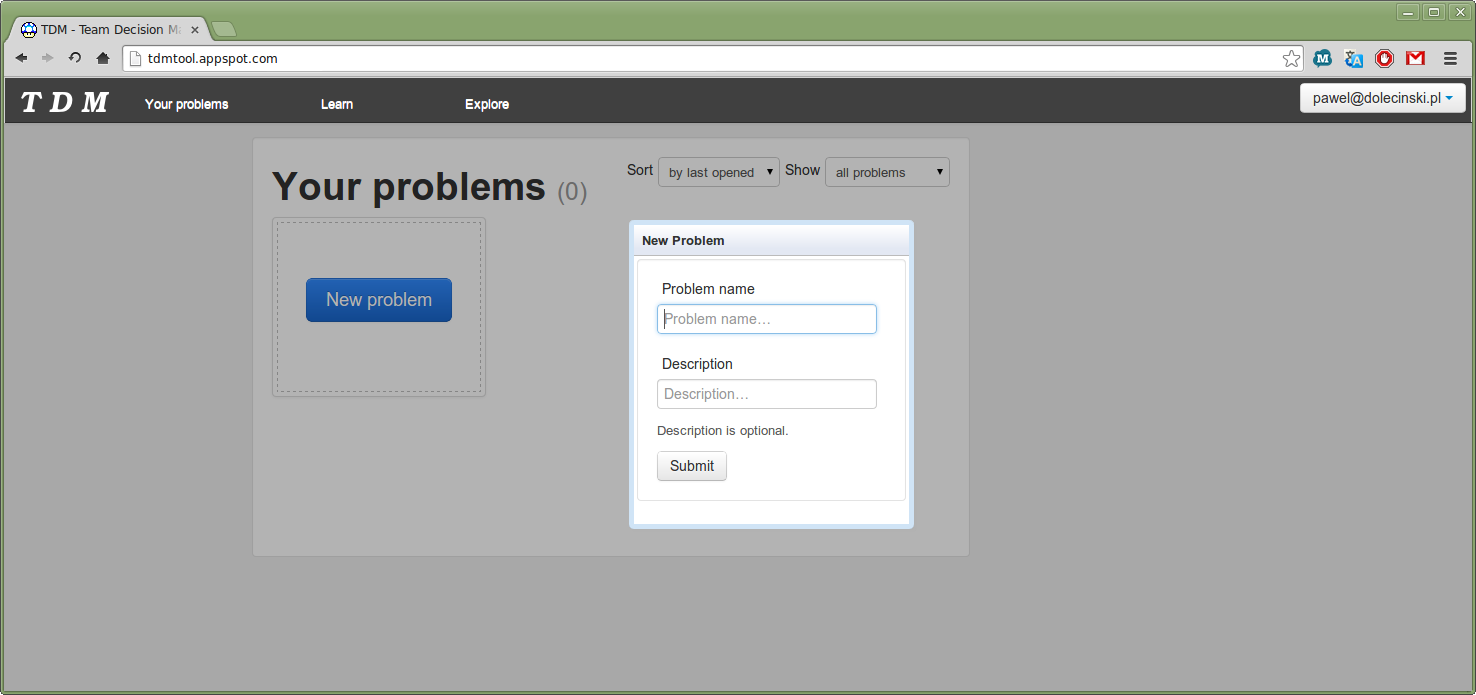
\includegraphics[width=\linewidth]
    {chapters/prototyp/tdm_new_problem}
  \caption{Okno dodawania nowego problemu decyzyjnego}
  \label{fig:new_problem}
\end{figure}

\subsubsection{Burza mózgów}
\begin{figure}[!htbp]
  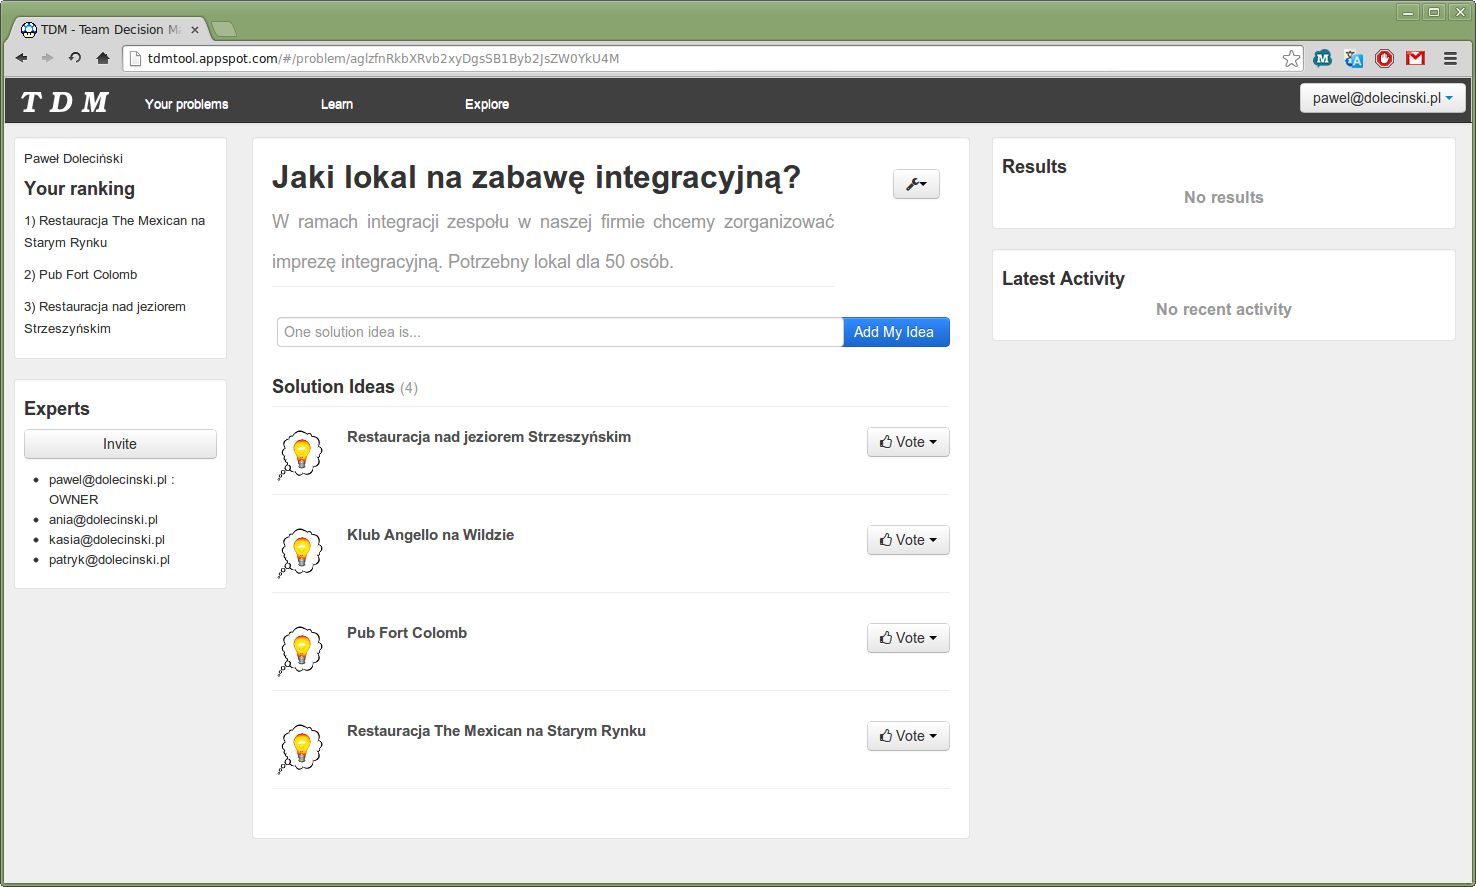
\includegraphics[width=\linewidth]
    {chapters/prototyp/tdm_brainstorm}
  \caption{Burza mózgów}
  \label{fig:brainstorm}
\end{figure}
Centralne miejsce aplikacji. To tutaj odbywa się cała dyskusja. Z poziomu ekranu
problemu decyzjnego jest dostęp do dodawania nowych alternatyw, komentowania,
głosowania. Widać aktualne wyniki oraz powiadomienia systemowe. Każdy z tych
elementów został omówiony bardziej szczegółowo w kolejnych sekcjach.

\subsubsection{Nowa alternatywa}
\missingfigure{Klient: nowa alternatywa}
Dodanie nowej alternatywy ogranicza się do wpisania kilku słów opisu i
naciśnięcia jednego przycisku. Natychmiast po tym propozycja rozsyłana jest do
pozostałych ekspertów, a na ekranie pojawia się dodatkowe okno z możliwością
bardziej szczegółowego przedstawienia swojego pomysłu. Jest tam miejsce na
dyskusję, która jest całkowicie anonimowa. Anonimowe jest też samo dodanie
alternatywy. Zabieg ten pomoga uniknąć ekspertom padnięcia ofiarami opisanego
wcześniej grupowego myślenia.

\subsubsection{Członkowie grupy}
Po lewej stronie widoku z ,,burzą mózgów'' widoczna jest lista wszystkich
uczestników dyskusji, czyli tak zwanych ekspertów. Zawsze jeden z członków grupy
jest wyróżniony. Jest to tak zwany właściciel, czyli osoba która stworzyła
problem. To do właściciela należy ostatnie słowo, czyli możliwość zakończenia
całego procesu w każdej chwili. Na liście członków grupy pokazywana jest też
aktualna dostępność każdej osoby.

Zaproszenie nowych ekspertów sprowadza się do podania adresów e-mail oraz kilku
słów zachęty. Na każdy z podanych adresów zostanie wysłana wiadomość e-mail z
zaproszeniem do udziału w dyskusji wraz z adresem dostępu. Wejście na podany
adres wymaga od użytkownika jedynie zalogowania do systemu, po czym od razu
możliwe jest uczestnictwo w procesie decyzyjnym.
\begin{figure}[!htbp]
  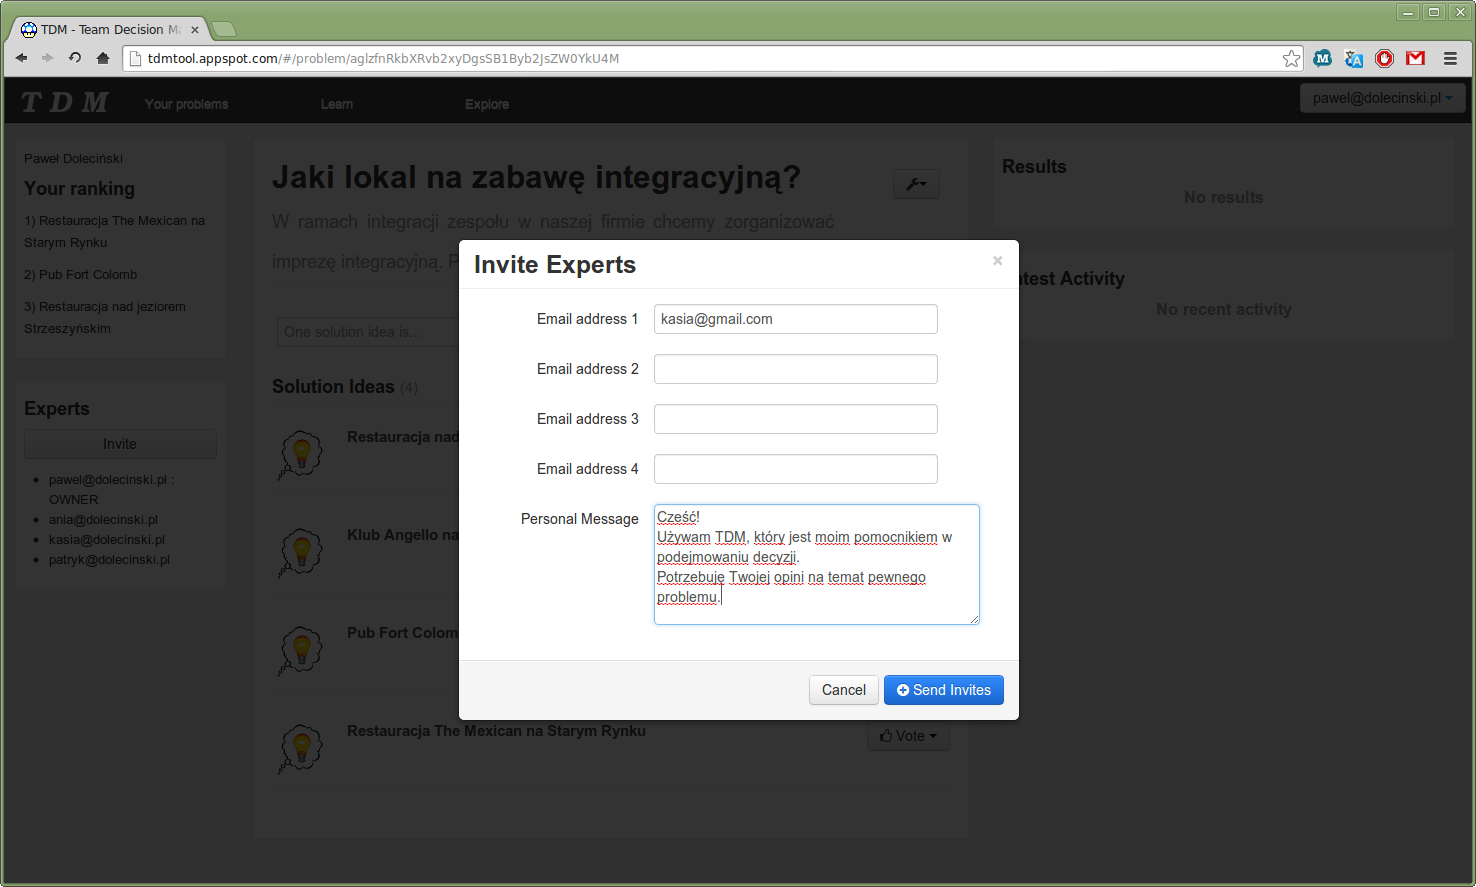
\includegraphics[width=\linewidth]
    {chapters/prototyp/tdm_invitation}
  \caption{Zapraszanie ekspertów}
  \label{fig:invitation}
\end{figure}
\missingfigure{Klient: głosowanie}
\subsubsection{Głosowanie i wyniki}
Ostatnim ważnym elementem prototypu klienta aplikacji TDM jest możliwość
wprowadzania swoich preferencji względem zaproponowanych alternatyw oraz,
prezentowane po prawej stronie widoku ,,burzy mózgów'', statystyki głosowań i
rekomendowane przez system rozwiązanie optymalne dla grupy.

\subsection{Serwer}
Serwer to serce projektu i jednocześnie podstawowa implementacja modelu systemu
grupowego podejmowania decyzji przedstawionego w poprzednim rozdziale. 

Całość zaimplementowana w języku Java i Scala, w oparciu o technologię JavaEE
oraz Spring Framework. Aplikacja TDM została wdrożona na Google App Engine,
platformie działającej jako chmura obliczeniowa udostępniona na
zasadzie platforma jako usługa (PaaS, ang. platform as a service).

Architektura serwera może być przedstawiona na dwa sposoby. Pierwszy to podział
na moduły logiczne odpowiadające modułom modelu teoretycznego. Drugi to podział
na warstwy przepływu danych oraz moduły odpowiedzialne za pracę w każdej z warstw.

\subsubsection{Moduły logiczne}
Przed szczegółowym opisem modułów warto wspomnieć, że użytkownik po wysłaniu
swoich preferencji nie czeka na odpowiedź serwera. Może kontynuować dyskusję,
zgłaszać nowe pomysły rozwiązań, a nawet wysłać nowe preferencje. Serwer sam
poinformuje o nowych wynikach głosowania jak tylko będzie gotowy. Dzięki temu
zachowana jest dynamika i naturalność dyskusji oraz całego procesu. Wszystkie
komunikaty wysyłane do serwera oraz zwracane przez serwer są całkowicie
asynchroniczne.

\begin{itemize}
  \item \emph{Moduł unifikowania preferencji}. Jest odpowiedzialny za
  zunifikowanie preferencji nadesłanych przez ekspertów przy użyciu funkcji
  transformacji zaproponowanych w modelu teoretycznym. Co prawda prototyp
  klienta TDM pozwala podać preferencje tylko przy pomocy funkcji użyteczności,
  jednak serwer w pełni obługuje wszystkie cztery możliwości oceny alternatyw.
  Ze względu na funkcyjną postać transformacji, cały moduł został
  zaimplementowany w języku Scala z rodziny języków dla maszyny wirtualnej Javy,
  który wspiera paradygmat programawania funkcyjnego. Zunifikowane preferencje
  zapisywane są w bazie danych lub, jeżeli dany użytkownik głosował już, to dane
  w bazie są nadpisywane bądź uzupełniane.

  \item \emph{Moduł selekcji}. Zaraz po zunifikowaniu ocen ekspertów, serwer
  przechodzi do fazy selekcji, czyli próby wyznaczenia najlepszego w danej
  chwili rozwiązania. Wyniki obliczeń propagowane są wśród wszystkich
  podłączonych w danym momencie aplikacji klienckich oraz zapisywana w bazie
  danych. Dodatkowo w bazie zapisywane są pośrednie wyniki, czyli zagregowana
  relacja preferencji oraz stopnie dominancji.

  \item \emph{Moduł konsensusu}. Zgodnie z metodami obliczeń z modelu
  sprawdzany jest poziom konsensusu grupy. Innymi słowy, ten fragment serwera
  odpowiedzialny jest za poinformowanie użytkowników czy mogą zakończyć
  dyskusję, czy jeszcze nie. Przeciwnie do innych systemów grupowego
  podejmowania decyzji, serwer TDM nie kończy całego procesu i nie podaje
  finalnego rozwiązania w przypadku osiągnięcia minimalnego poziomu konsensusu.
  Rozsyłana jest jedynie informacja, że taki poziom został osiągnięty wraz z
  sugestią zakończenia. Każdorazowo moduł rozsyła także statystyki dotyczące
  głosowań, czyli ilu z zaproszonych ekspertów wyraziło swoje zdanie i w jakim
  stopniu to zdanie jest kompletne.

  \item \emph{Moduł informacji zwrotnej}. Jeżeli nie został osiągnięty minimalny
  poziom konsesusu, to moduł ten będzie się starał ,,pchnąć'' użytkowników w
  stronę osiągnięcia tego poziomu. Na podstawie danych zebranych w poprzednich
  modułach generowane są rekomendacje dla eksperta, który nadesłał preferencje.
  O ile moduł selekcji i moduł konsensusu rozsyłają wyniki obliczeń do
  wszystkich aktywnych użytkowników, o tyle moduł informacji zwrotnej wysyła
  rekomendacje jako odpowiedź na nadesłane preferencje.

  \item \emph{Moduł zarządzania problemami}. Część systemu niewchodząca w skład
  samego modelu teoretycznego, jednak niezbędna do pracy całości. Jest to moduł
  odpowiedzialny za tworzenie, pobieranie, archwizację problemów. 
   
\end{itemize}
\subsubsection{Architektura trójwarstwowa}
Architektura trójwarstwowa (ang. three-tier architecture) to koncepcja, w której
interfejs użytkownika, przetwarzanie danych i składowanie danych są rozwijane w
postaci osobnych modułów. Prototyp serwera TDM jest zaimplementowany właśnie w
taki sposób.

\begin{description}
  \item[Warstwa interfejsu użytkownika] (ang. presentation
  layer) zaimplementowana z użyciem biblioteki Spring MVC jest odpowiedzialna za
  bezpośrednią komunikację z klientem.
  Nasłuchuje na żądania, po wstępnej walidacji i transformacji przesyła dane do
  niższej warstwy. Komunikacja przebiega tak samo w drugą stronę, to znaczy
  kiedy warstwa logiki aplikacji posiada dane dla klienta, to warstwa interfejsu
  użytkownika odpowiada za wysłanie tych danych. Na tym poziomie zdefiniowany
  jest protokół komunikacji REST oraz serializacja/deserializacja obiektów
  języka Java do formatu JSON (ang. JavaScript Object Notation).
  
  \item[Warstwa przetwarzania danych] zwana inaczej warstwą logiki biznesowej
  (ang. business logic layer). Opisane wcześniej moduły logiczne
  zaimplementowane są właśnie na tym poziomie. Jest to warstwa, która skupia się
  na samym modelu i logice bez wchodzenia w szczegóły techniczne wykorzystywanej
  technologii. Dzięki temu w każdym momencie możliwa jest łatwa zmiana protokołu
  komunikacji z klientem albo zmiana wykorzystywanej bazy danych lub serwera.
  Łatwiejsze i wygodniejsze jest także testowanie samego modelu.
  
  \item[Warstwa składowania danych] zwana inaczej warstwą persystencji (ang.
  persistance layer). Najniższa warstwa, odpowiedzialna za zapis wyników
  obliczeń i danych pochodzących z warstwy logiki biznesowej. Prototyp TDM z
  uwagi na wykorzystanie Google App Engine, korzysta z obiektowej bazy danych
  zamiast tradycyjnej relacyjnej, co daje elastyczny i łatwo rozszerzalny
  schemat bazy. Jednocześnie nie jest potrzebna bezpośrednia komunikacja z bazą
  danych, ponieważ został użyty standard persystencji obiektów Javy JDO (ang.
  Java Data Objects), który jest niezależny od dostawcy wykorzystywanej bazy.
\end{description}
Jak widać, cały serwer jest bardzo mocno zmodularyzowany, co pozwala na duże
możliwości rozszerzania o nowe funkcjonalności oraz w przyszłości zmiany
wykorzystywanych technologii na nowsze.

\section{Studium przypadku}
W tym podrozdziale zilustrowany jest prosty, ale prawdziwy przykład
wykorzystania systemu wpierania decyzji grupowej. Warto zwrócić uwagę na
zachowanie systemu w przypadku złożonych problemów, kiedy to zbiór alternatyw
może bardzo się zmieniać w krótkich odstępach czasu, jak również zbiór ten może
być bardzo duży. Model systemu nie nakłada żadnych ograniczeń ilościowych na
alternatywy, może też obsługiwać dowolną liczbę ekspertów. Aby pokazać działanie
prototypu, będziemy śledzić przepływ informacji przedstawiony wcześniej.

Jako studium przypadku została wybrana grupa czterech osób - współpracowników,
którzy muszą wybrać lokal na spotkanie integracyjne. Wszyscy na co dzień
pracują w różnych krajach i w różnych strefach czasowych, co uniemożliwia
wspólne spotkanie w celu dokonania wyboru.

W pierwszej kolejności jeden z członków grupy (zwany dalej moderatorem) musi
stworzyć nowy problem w aplikacji TDM. Trzeba podać nazwę problemu oraz
opcjonalalnie opis wyjaśniający problem. Następnie, aby proces miał sens, trzeba
podać przynajmniej dwie alternatywy oraz zaprosić do dyskusji pozostałe osoby. W
tym przykładzie na początku dostępnych jest pięć propozycji lokali zebranych w
tabeli \ref{tab:init_ideas}.
\missingfigure{screenshot z aplikacji: dodanie idei oraz ekspertow}
Aplikacja samodzielnie inicjalizuje niezbędne dla obliczeń parametry problemu
decyzyjnego. Samodzielnie można zmienić maksymalny podzbiór alternatyw brany pod
uwagę, który domyślnie przyjmuje wartość nieskończoną. Dla prostoty przykładu
oraz lepszego pokazania dynamiki alternatyw maksymalny podzbiór alternatyw
ustawiony jest na 4. Wszystkie wartości parametrów zebrane zostały w tabeli
\ref{tab:init_problem_params}.

\begin{table}[ht]
\caption{Początkowe propozycje rozwiązania problemu}
\begin{tabularx}{\textwidth}{|c|c|X|}
\hline
ID & Nazwa & Opis \\
\hline
$x_1$ & Lokal 1 & Miejsca: $75$ Cena: $100\textrm{zł}$ \\
\hline
$x_2$ & Lokal 2 & Miejsca: $50$ Cena: $90\textrm{zł}$ \\
\hline
$x_3$ & Lokal 3 & Miejsca: $60$ Cena: $120\textrm{zł}$ \\
\hline
$x_4$ & Lokal 4 & Miejsca: $100$ Cena: $60\textrm{zł}$ \\
\hline
$x_5$ & Lokal 5 & Miejsca: $75$ Cena: $70\textrm{zł}$ \\
\hline
\end{tabularx}
\label{tab:init_ideas}
\end{table}

\begin{table}[ht]
\caption{Początkowe parametry problemu}
\begin{tabularx}{\textwidth}{|c|c|X|}
\hline
Nazwa & Wartość & Opis \\
\hline
b & 1 & Kontroluje rygorystyczność procesu przy obliczaniu miar bliskości \\
\hline
$\beta$ & 0.5 & kontroluje zachowanie OR-LIKE operatora agregacji \\
\hline
minConsDegree & 0.8 & Minimalny poziom konsensusu \\
\hline
minProxDegree & 0.7 & Minimalny poziom bliskości \\
\hline
minQGDD & 0.2 & Minimalny poziom dominancji \\
\hline
DSsize & 4 & Maksymalny podzbiór alternatyw \\
\hline
\end{tabularx}
\label{tab:init_problem_params}
\end{table}

Należy zwrocić uwagę, że początkowy zbiór wszystkich rozwiązań składa się z
pięciu lokali $\mathcal{X} = \{ x_1, x_2, x_3, x_4, x_5\}$, natomiast założono,
że eksperci powinni w jednym momencie skupić się na ocenie maksymalnie czterech.
Zatem początkowy podzbiór rozwiązań składa się tylko z pierwszych czterech
zaproponowanych $\mathcal{X'} = \{ x_1, x_2, x_3, x_4\}$.

Dla uproszczenia obliczeń oraz ze względu na ograniczoną ilość miejsca w tej
pracy, pokazane zostaną tylko dwie ,,rundy''. Zakładamy też, że każda runda na
wejściu otrzymuje kompletny zbiór preferencji od każdego z ekspertów. 
Warto natomiast pamiętać, że cały proces uruchamiany jest każdorazowo dla
pojedynczego głosu. 

\subsection{Pierwszy etap w procesie decyzyjnym}
Na rysunku pokazane są preferencje ekspertów wyrażone za pomocą funkcji
użyteczności.

\subsubsection{Etap unifikowania}
W pierwszej kolejności preferencje podane przez ekspertów muszą zostać poddane
unifikacji, czyli wyrażone za pomocą rozmytej relacji preferencji. Moduł
unifikowania wykorzystuje wzory transformacji opisane w modelu teoretycznym, co
daje następujące wyniki:
$$
P^1 = 
\begin{pmatrix}
0.5  & 0.16  & 0.33  & 0    \\
0.83 & 0.5   & 0.66  & 0.33 \\
0.66 & 0.33  & 0.5   & 0.16 \\
1    & 0.66  & 0.83  & 0.5
\end{pmatrix},\;
P^2 = 
\begin{pmatrix}
0.5  & 0.57  & 0.88  & 0.94 \\
0.43 & 0.5   & 0.84  & 0.92 \\
0.22 & 0.16  & 0.5   & 0.69 \\
0.06 & 0.08  & 0.21  & 0.5
\end{pmatrix},
$$

$$
P^3 = 
\begin{pmatrix}
0.5  & 0.3   & 0.9   & 0.7  \\
0.7  & 0.5   & 1     & 0.8  \\
0.1  & 0     & 0.5   & 0.2  \\
0.3  & 0.2   & 0.8   & 0.5
\end{pmatrix},\;
P^4 = 
\begin{pmatrix}
0.5  & 0.66  & 0.97  & 0.82 \\
0.34 & 0.5   & 0.91  & 0.66 \\
0.03 & 0.09  & 0.5   & 0.18 \\
0.18 & 0.34  & 0.82  & 0.5
\end{pmatrix}.
$$
  
\subsubsection{Proces selekcji}
Wykorzystując kryterium rozmytej większości oraz operator OWA z wektorem wag
$W= [0.5,0.2,0.17,0.13]$ (,,większość''), w fazie agregacji obliczana jest
zbiorowa rozmyta relacja preferencji:
$$
P^c = 
\begin{pmatrix}
0.5  & 0.52  & 0.86   & 0.7  \\
0.48 & 0.5   & 0.91   & 0.8  \\
0.14 & 0.09  & 0.5    & 0.2  \\
0.25 & 0.23  & 0.56   & 0.5
\end{pmatrix}.
$$

Następnie moduł eksploatacji przedstawi proponowane rozwiązanie problemu. 
W oparciu o operator OWA z wektorem wag $W = [0.07, 0.67, 0.26]$
(,,większość'') obliczane są stopnie dominancji (QGDD): $QGDD_1 = 0.696$,
$QGDD_2 = 0.702$, $QGDD_3 = 0.146$, $QGDD_4 = 0.265$. Są to wartości, które
reprezentują dominancje jaką jedna alternatywa ma nad ,,większością''
pozostałych alternatyw według ,,większości'' ekspertów.

Na podstawie powyższych wyników widać, że obecnie najlepszym kandydatem jest
lokal drugi $x_2$, a tymczasowe rozwiązanie można zaprezentować jako
uporządkowaną listę $\{ x_2, x_1,x_4, x_3\}$.

\subsubsection{Proces konsensusu}
Pierwszy krok został już osiągniety. System może przedstawić proponowane
rozwiązanie na podstawie zgłoszonych preferencji ekspertów. Ale to nie koniec. W
module konsensusu system musi sprawdzić w jakim stopniu eksperci są zgodni ze
sobą, tzn. czy zaproponowane wyżej rozwiązanie jest rozwiązaniem odpowiadającym
większości grupy.

Najpierw moduł musi ustalić indywidualne dla każdego eksperta uporządkowanie
alternatyw na tej samej zasadzie, co obliczanie zbiorczego rozwiązania:
$$e_1: \{ x_4, x_2, x_3, x_1 \}, \;\; e_2: \{ x_1, x_2, x_3, x_4 \},$$
$$e_3: \{ x_1, x_2, x_4, x_3 \}, \;\; e_4: \{ x_2, x_1, x_4, x_3 \}.$$

Stopnie konsensusu dla każdej z alternatyw to: $C(x_1) = 0.55, C(x_2) =
0.66,$ $C(x_3) = 0.77, C(x_4) = 0.66.$ Miara konsensusu wynosi
$C_{\mathcal{X}} = 0.67$.
Ostatecznie obliczone miary bliskości wynoszą: $P^1_{\mathcal{X}} = 0.55,\;
P^2_{\mathcal{X}} = 0.67,\; P^3_{\mathcal{X}} = 0.78,\; P^4_{\mathcal{X}} = 1$.

Jasno widać, że konsensus nie osiągnął wymaganej wartości minimalnej
($C_{\mathcal{X}} < 0.8$), czyli aplikacja powinna kontynuować kolejne etapy,
szczególnie etap generowania informacji zwrotnej.

\subsubsection{Dynamiczny wybór alternatyw}
Eksperci w każdym momencie działania aplikacji mogą zgłaszać nowe alternatywy,
mogą również zgłosić, że jedna z opcji brana do tej pory pod uwagę jest już
nieaktualna, na przykład jeden z lokali ma już komplet rezerwacji.
W tej sytuacji niezbędna jest aktualizacja wszystkich danych o problemie, które
mogły się zmienić w trakcie działania procesu.

W tym przypadku okazało się, że alternatywa $x_3$ nie osiągnęła minimalnego
stopnia dominancji, t.j. $QGDD_3 < MinQGDD = 0.2$. W międzyczasie zgłoszona
została nowa propozycja $x_6$. System zgłasza usunięcie $x_3$ z
podzbioru dyskusji oraz dołączenie w to miejsce $x_6$. Jest jeszcze jedna
oczekująca alternatywa $x_5$, jednak aplikacja w pierwszej kolejności promuje
najnowsze propozycje ekspertów. W przypadku większej ilości propozycji istnieje
możliwość wstępnego głosowania na nowe opcje. Inną możliwością jest zwiększenie
rozmiaru podzbioru dyskusji.

\subsubsection{Informacja zwrotna}
Moduł informacji zwrotnej jest odpowiedzialny za doprowadzanie grupy do jak
największego konsensusu. Zatem generowane są rekomendacje oraz podpowiedzi dla
każdego członka, który nie zgadza się z większością. Oczywiście są to tylko
wskazówki, których nie trzeba stosować.

Aplikacja najpierw szereguje ekspertów według osiągniętych przez nich miar
bliskości: $e_4, e_3, e_2, e_1$. W tym momencie widać, że dwóch członków grupy,
$e_2$ i $e_1$, uzyskało poziom bliskości poniżej minimalnego $minProxDegree$,
zatem oni zostaną poproszeni o zmianę swoich preferencji. Oczywiście
rekomendacje na temat propozycji $x_3$ są pomijane ze względu na jej usunięcie.
Natomiast wszyscy eksperci są proszeni o podanie swoich preferencji dla nowej
alternatywy $x_6$. Rekomendacje otrzymane przez ekspertów można zobaczyć na
rysunku. \missingfigure{Rekomendacje dla ekspertów}

\subsection{Drugi etap w procesie decyzyjnym}
Jest to faza, w której wszyscy eksperci ponownie wysłali swoje preferencje dla
wszystkich alternatyw w oparciu o rekomendacje. Wszystkie preferencje zostały
zebrane na rysunku. \missingfigure{Rekomendacje dla ekspertów}

Cały proces z rundy pierwszej jest powtarzany, tzn. preferencje są
transformowane do rozmytych relacji preferencji, a moduł selekcji przedstawia
nowe rozwiązanie problemu. Nowy ranking lokali to $x_2, x_1, x_6, x_4$.

Następnie moduł konsensusu sprawdza osiągnięty poziom porozumienia. Dla podanych
danych przykładowych otrzymano $C_{\mathcal{X}} = 0.88$. Oznacza to, że został
osiągnięty minimalny poziom wymagany przez problem ($C_{\mathcal{X}} > 0.8$),
a grupa zostaje zapoznana z proponowanym rozwiązaniem. Aplikacja informuje, że
większość członków grupy zgadza się ze sobą, ale nic nie stoi na przeszkodzie w
kontynuowaniu dyskusji - decyzja zawsze należy do grupy.

